\chapter{\label{chap:chap3}{Planning}}

According to \cite{Kitchenham_2007}, a systematic literature review is a means of identifying, evaluating, and interpreting all available research relevant to a particular research question, topic area, or phenomenon of interest. The most common reasons for undertaking it are described below:

\begin{enumerate}
\item Summarize the existing evidence concerning a treatment or technology; 
\item Identify any gaps in current research in order to suggest areas for further investigation; 
\item Provide a framework/background in order to appropriately position new research activities.
\end{enumerate}

The current work is motivated by the first item, as it aims to summarize the \textit{state of the art} on how acceptance tests are measured regarding their quality.

\section{Review Process}

We follow the three stages that \cite{Kitchenham_2007} described to define the current work phases, as follows:

\begin{enumerate} 
\item Planning stage, covered on Chapter \ref{chap:chap4}
    \begin{enumerate}
    \item Specifying the research question(s)
    \item Developing a review protocol
    \end{enumerate}
\item Execution stage, covered on Chapter \ref{chap:chap5}
    \begin{enumerate}
    \item Identification of research
    \item Selection of primary studies
    \item Study quality assessment
    \item Data extraction and monitoring
    \item Data synthesis
    \end{enumerate}
\item Reporting stage, covered on Chapter \ref{chap:chap6}
    \begin{enumerate}
    \item Formatting the main report 
    \item Evaluating the report 
    \end{enumerate}
\end{enumerate}

\section{Review process timetable}

Based on the before mentioned stages, a timetable was defined as follows below

\begin{figure}[!h]
\centering
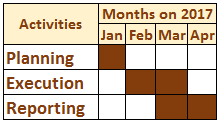
\includegraphics[scale=1]{images/planning}
\caption{Review process timetable}
\label{fig:planning}
\end{figure}